\section{Neutron Irradiation}
\label{sec:irradiation}

\subsection{Rhode Island Neutron Irradiation Facility}
\label{subsec:RINSC}
RINSC (Rhode Island Nuclear Science Center) is a 2 MW, light water cooled, pool type reactor in Narragansett, Rhode Island, USA.
\begin{itemize}
    \item Fig 1 - image(s) of reactor core, beamport (see fig~\ref{fig:RINSC_Facility})
    \item Fig 2 - puck design/layout, real pucks
    \item Fig 3 - puck layout, packing
    \item Fig 4 - other hardware, cylinder, temp monitoring setup
    \item Fig 5 - schemaitc of experimental setup? Is this needed?
\end{itemize}

  \begin{figure}[!hbt]
  \begin{center}
    \includegraphics[width=0.80\textwidth]{figures/RINSC_Reactor_Core}
    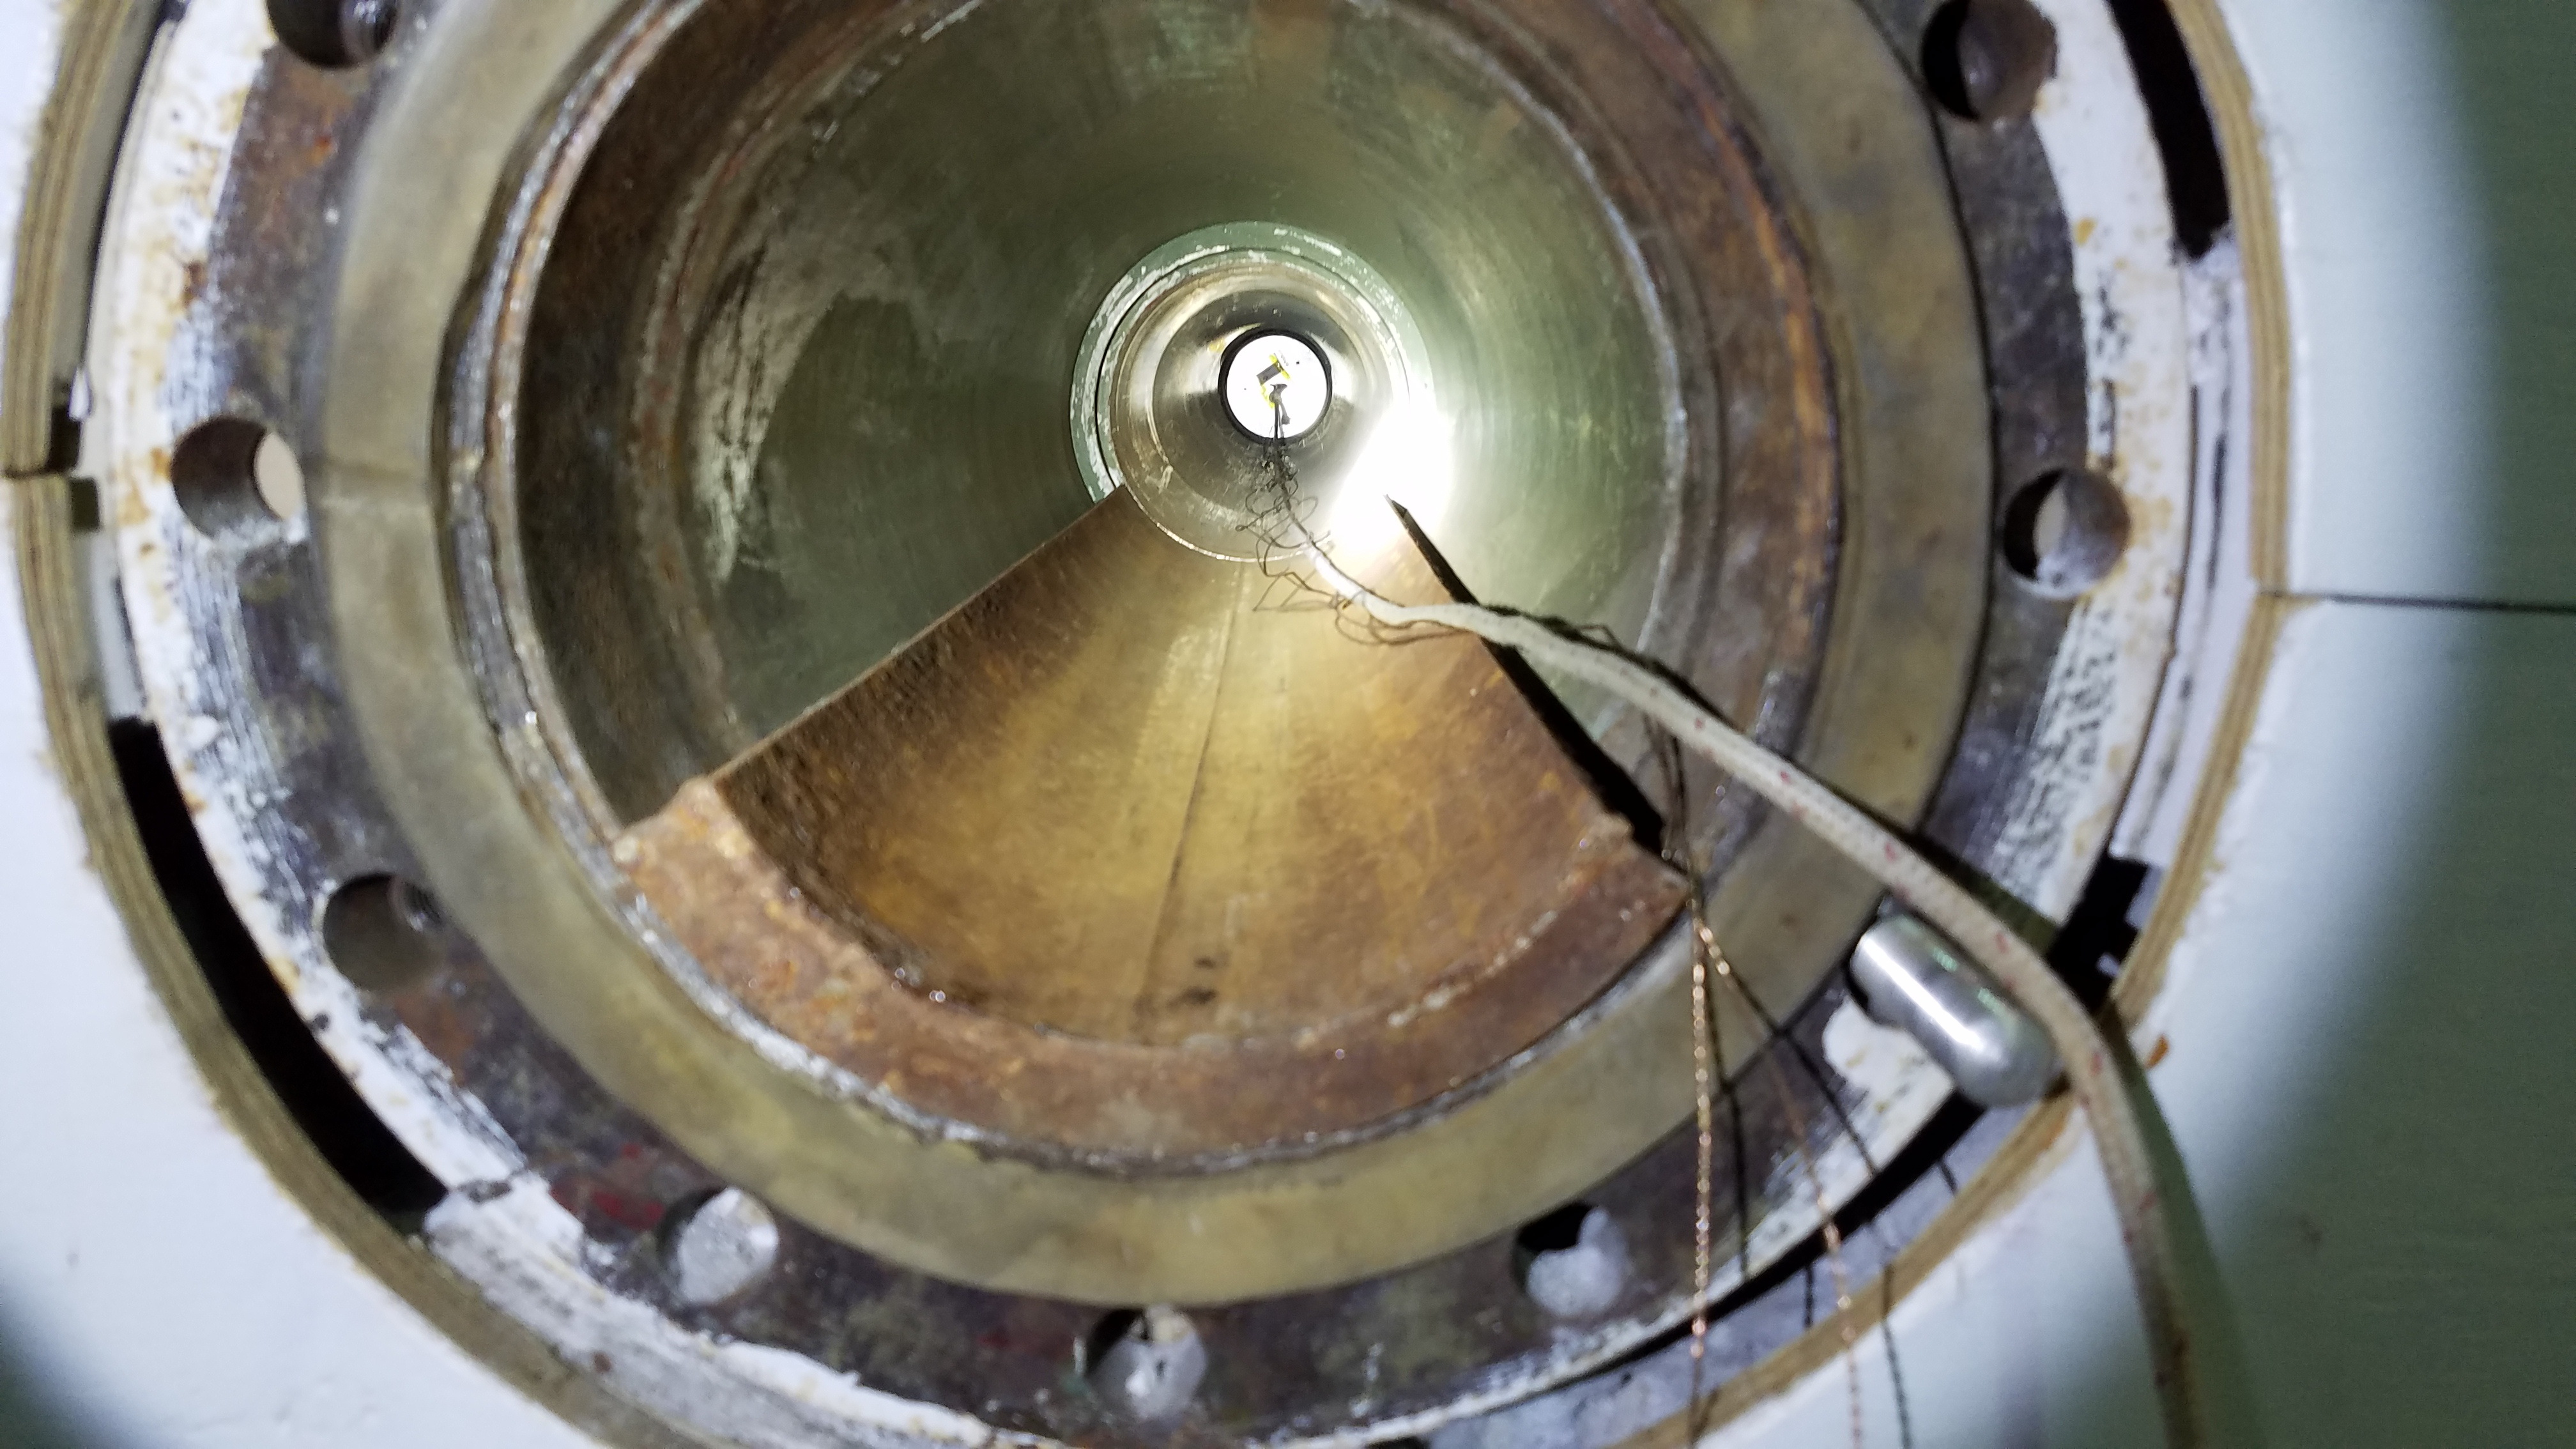
\includegraphics[width=0.80\textwidth]{figures/Beamport_View}
    \caption{On the left is an image of the reactor core at RINSC, and on the right is a view down the beamport used for these irradiation studies.}
    \label{fig:RINSC_Facility}
  \end{center}
\end{figure}


\subsection{List of Neutron-Irradiated Sensors}
\label{subsec:sensors_irradiation}
